\documentclass{lecturefig}
\usetikzlibrary{chains}
\begin{document}
\begin{frame}[fragile]
  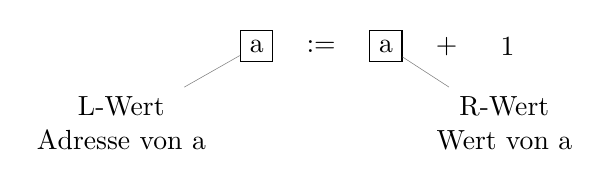
\begin{tikzpicture}[start chain, node distance=3mm]
    \node[on chain,draw,pin={[align=center]-135:{\structure{L-Wert}\\Adresse von a}}] (a)    {a};
    \node[on chain] (eq)   {:=};
    \node[on chain,draw,pin={[align=center]-45:{\structure{R-Wert}\\Wert von a}}] (b)    {a};
    \node[on chain] (plus) {+};
    \node[on chain] (one) {1};

  \end{tikzpicture}
\end{frame}
\end{document}
